% =========================================================
%  MIDTERM REPORT: AIRLINE BOOKING DATA CLEANING & ANALYSIS
%  Course: Data Analytics
%  Project: Aurora Air & Horizon Wings (Period: 2024--2026)
% =========================================================
\documentclass[12pt, a4paper]{report}

% ---- Character Encoding & Language Configuration ----
\usepackage{iftex}
\ifPDFTeX
  \usepackage[T5]{fontenc}
  \usepackage[utf8]{inputenc}
  \usepackage[vietnamese,english]{babel}
\else
  \usepackage{fontspec}
  \usepackage[vietnamese,english]{babel}
\fi

% ---- Academic Typography ----
\usepackage{mathpazo}            % Palatino for body text
\usepackage[scaled=0.92]{helvet} % Helvetica for sans-serif headings
\usepackage{courier}             % Courier for inline code

% ---- Page Margins ----
\usepackage[
  top=2.5cm, bottom=2.5cm,
  left=3.0cm, right=2.5cm,
  headheight=15pt
]{geometry}

% ---- Line Spacing & Paragraph Formatting ----
\usepackage{microtype}
\usepackage{setspace}
\setstretch{1.25}
\usepackage{parskip}
\setlength{\parindent}{0pt}

% ---- Mathematics & Symbols ----
\usepackage{amsmath, amssymb}

% ---- Academic Color Palette ----
\usepackage[table]{xcolor}
\definecolor{NavyBlue}{RGB}{0,40,100}
\definecolor{DarkSlate}{RGB}{35,70,105}
\definecolor{LightGray}{RGB}{242,244,248}
\definecolor{AccentRed}{RGB}{180,35,35}
\definecolor{AccentGreen}{RGB}{25,120,70}
\definecolor{AccentOrange}{RGB}{205,105,20}
\definecolor{TableHead}{RGB}{215,230,248}
\definecolor{TableAlt}{RGB}{246,249,254}
\definecolor{InsightBg}{RGB}{238,245,254}
\definecolor{BoxBorder}{RGB}{45,95,150}

% ---- Tables ----
\usepackage{booktabs}
\usepackage{tabularx}
\usepackage{longtable}
\usepackage{multirow}
\usepackage{array}
\usepackage{makecell}

% ---- Graphics & Visualization ----
\PassOptionsToPackage{final}{graphicx}
\usepackage[final]{graphicx}
\makeatletter
\Gin@draftfalse
\makeatother
\setkeys{Gin}{draft=false}
\usepackage{float}
\usepackage[font={small,sf}, labelfont={bf,color=NavyBlue}, skip=8pt]{caption}
\usepackage{subcaption}
\DeclareGraphicsExtensions{.png,.jpg,.jpeg,.pdf}
\graphicspath{{figures/}{./}}

% ---- Caption Labels (English Standard) ----
\addto\captionsenglish{%
  \renewcommand{\tablename}{Table}%
  \renewcommand{\figurename}{Figure}%
}

% ---- Indented Lists ----
\usepackage{enumitem}
\setlist[itemize]{noitemsep, topsep=4pt, leftmargin=1.5em}
\setlist[enumerate]{noitemsep, topsep=4pt, leftmargin=1.5em}

% ---- Running Headers & Footers ----
\usepackage{fancyhdr}
\pagestyle{fancy}
\fancyhf{}
\fancyhead[L]{\small\sffamily\textit{Midterm Report --- Airline Booking Data Analysis}}
\fancyhead[R]{\small\sffamily\textit{Aurora Air \& Horizon Wings}}
\fancyfoot[C]{\sffamily\thepage}
\renewcommand{\headrulewidth}{0.4pt}

% ---- Chapter & Section Formatting ----
\usepackage{titlesec}
\titleformat{\chapter}[block]
  {\normalfont\Large\bfseries\sffamily\color{NavyBlue}}
  {CHAPTER \thechapter.}{0.8em}{}[\vspace{0.3em}{\color{NavyBlue}\hrule height 1pt}\vspace{0.5em}]
\titlespacing*{\chapter}{0pt}{-10pt}{15pt}
\titleformat{\section}
  {\normalfont\large\bfseries\sffamily\color{NavyBlue}}
  {\thesection.}{0.5em}{}
\titleformat{\subsection}
  {\normalfont\normalsize\bfseries\sffamily\color{DarkSlate}}
  {\thesubsection.}{0.5em}{}

% ---- Hyperlinks ----
\usepackage[
  colorlinks=true,
  unicode=true,
  linkcolor=NavyBlue,
  citecolor=NavyBlue,
  urlcolor=DarkSlate,
  bookmarks=true,
  pdftitle={Airline Booking Data Cleaning & Analysis Report},
  pdfauthor={Data Analytics Research Team}
]{hyperref}

% ---- Insight & Recommendation Callout Box ----
\usepackage{tcolorbox}
\tcbuselibrary{skins, breakable}

\newtcolorbox{insightbox}[2][]{
  enhanced,
  breakable,
  colback=InsightBg,
  colframe=BoxBorder,
  fonttitle=\bfseries\sffamily,
  coltitle=white,
  title={#2},
  left=9pt, right=9pt,
  top=8pt, bottom=8pt,
  boxrule=0.8pt,
  arc=3pt,
  #1
}

% ---- Custom Macros ----
\newcommand{\code}[1]{\texttt{\small\color{DarkSlate}#1}}
\newcommand{\airline}[1]{\textbf{\textsf{#1}}}
\newcommand{\pct}[1]{\textbf{#1\%}}

% =========================================================
\begin{document}
% =========================================================
\renewcommand{\tablename}{Table}
\renewcommand{\figurename}{Figure}

% ---- ACADEMIC TITLE PAGE ----
\begin{titlepage}
  \centering
  \vspace*{1.0cm}

  {\large\sffamily\bfseries\color{NavyBlue}
    NATIONAL ECONOMICS UNIVERSITY --- FACULTY OF DATA SCIENCE\\
    COURSE: DATA ANALYTICS\\[0.4em]
  }

  \vspace{1.5cm}
  {\color{NavyBlue}\rule{\textwidth}{2pt}}\\[0.6em]

  {\LARGE\sffamily\bfseries\color{NavyBlue}
    MIDTERM REPORT\\[0.3em]
    AIRLINE BOOKING DATA CLEANING \& ANALYSIS
  }\\[0.6em]

  {\large\sffamily\color{DarkSlate}
    Empirical Study of Simulated Booking Behavior: \airline{Aurora Air} \& \airline{Horizon Wings}\\
    Collection Period: 2024\,--\,2026
  }

  {\color{NavyBlue}\rule{\textwidth}{2pt}}

  \vspace{2.0cm}

  \begin{tabular}{@{}ll@{}}
    \toprule
    \textbf{Project Team}          & Data Analytics Research Team \\
    \midrule
    \textbf{Team Members}       & Trần Thế Tùng --- Preprocessing \& Data Engineering \\
                                     & Tạ Minh Quân --- Database Administration \& QA \\
                                     & Nguyễn Đình Phan Anh --- BI \& Data Visualization \\
    \midrule
    \textbf{Snapshot Date}       & 15 September 2026 \\
    \textbf{Raw Dataset}      & 10,325 records $\times$ 24 fields \\
    \textbf{Analysis Dataset} & 10,000 unique bookings $\times$ 30 fields \\
    \bottomrule
  \end{tabular}

  \vfill
\end{titlepage}

% ---- TABLE OF CONTENTS ----
\tableofcontents
\clearpage

% =========================================================
\chapter{OVERVIEW, BUSINESS CONTEXT \& DATA SOURCES}
% =========================================================

\section{Business Context}

In modern commercial aviation, \textbf{Revenue Management} plays a central role in balancing ticket yield maximization against cabin seat occupancy (\textit{load factor}). Any mismatch between demand forecasts and actual flight operations can create material economic losses: overpricing results in perishable empty seats whose value vanishes at departure, whereas underpricing or weak reservation controls can trigger artificial overbooking and elevated cancellation rates.

This project investigates reservation behavior across two airlines representing distinct operating models:

\begin{itemize}
  \item \airline{Aurora Air:} Represents a traditional Full-Service Carrier (FSC). The airline operates an extensive route network with a multi-tier cabin configuration spanning Economy (E1, E2, E3, E4), Premium Economy (P1, P2), Business (B1, B2, B3), and First Class (F1, F2, F3). Its target customer base exhibits high service sensitivity and expects strong reliability alongside bundled amenities.

  \item \airline{Horizon Wings:} Represents a next-generation carrier operating with a flexible, cost-optimized business model. It targets leisure travelers, family/group itineraries (Group), and large Corporate Contract accounts by competing on convenience and competitive fares.
\end{itemize}

Airline reservation data captures the end-to-end transaction lifecycle: ticketing timestamps, booking horizon (\textit{lead time}), customer segments, distribution channels, and final operational status (\textit{Flown, Cancelled, No-Show}). Rigorous analysis of this dataset provides the analytical foundation for optimizing inventory release schedules, dynamic pricing structures, and proactive cancellation risk mitigation.

\section{Research Objectives}

This study is designed around three core objectives:

\begin{enumerate}
  \item \textbf{Systematic Data Cleaning and Full Lineage Traceability (100\% Lineage):} Design and execute an automated Python preprocessing pipeline that resolves exact duplicates, normalizes numeric anomalies, reconciles business-logic conflicts, and guarantees that the lineage table \code{row\_lineage.csv} accounts for all 10,325 raw records with zero information loss.

  \item \textbf{Database Schema Standardization:} Produce the standardized clean dataset \code{reservations\_clean.csv} containing exactly 10,000 unique bookings, enrich it with 7 business-derived columns, and compile a monthly operational summary table in \code{monthly\_summary.csv}.

  \item \textbf{Empirical Analysis and Managerial Implications:} Quantitatively address nine analytical business questions (Questions 2--10), examine how operational attributes associate with cancellation risk, and synthesize six actionable business insights to support executive decision-making.
\end{enumerate}

\section{Data Source Description and System Anomaly Profile}

The input dataset \code{data/airline\_bookings\_dirty.csv} contains \textbf{10,325 transaction records $\times$ 24 fields}, capturing bookings with departure dates spanning July 2024 through August 2026. All analyses in this report are anchored to the system cut-off date (\textit{Snapshot Date}) of \textbf{15 September 2026}.

Technical auditing reveals that the raw dataset mirrors common data integrity errors arising during synchronization across Global Distribution Systems (GDS), Online Travel Agencies (OTAs), and airline reservation hosts:
\begin{itemize}
  \item \textbf{Duplicate Records:} 416 rows are involved in exact duplicates across the 23 attribute columns (containing 208 redundant duplicate copies), and 117 rows share a \code{reservation\_id} while holding fragmented attribute values across rows.
  \item \textbf{Mixed Date Formats:} Four heterogeneous date formats coexist across records (\code{YYYY-MM-DD}, \code{DD/MM/YYYY}, \code{Month DD, YYYY}, and \code{DD-Mon-YYYY}).
  \item \textbf{Column Misalignment:} Date values were inadvertently shifted into the status string field \code{booking\_status}.
  \item \textbf{Text and Unit Contamination:} Quantitative fields contain trailing text units (\textit{days, pax, requests}), while fare columns mix currency symbols (\$, USD, EUR) and thousand-separator commas.
  \item \textbf{Business-Logic Contradictions:} 42 records exhibit a mismatch between the cancellation flag \code{is\_cancelled} and the observed operational status \code{booking\_status}.
\end{itemize}

% =========================================================
\chapter{DATA QUALITY AUDIT \& PREPROCESSING PIPELINE}
% =========================================================

\section{Initial Data Quality Assessment}

Prior to applying any data transformations, the team conducted a structural audit across all 10,325 raw records. This survey quantified missingness across each attribute and cataloged \textbf{12 core data quality issues} (\code{a\_issue\_catalog.csv}).

\subsection{Missingness Profile Across Key Attributes}

Missingness statistics are summarized in Table \ref{tab:missing_survey}, distinguishing true empty fields from non-standard junk placeholders.

\begin{table}[H]
  \centering
  \caption{Missing Data Statistics Across Key Attributes ($N = 10,325$ Records)}
  \label{tab:missing_survey}
  \renewcommand{\arraystretch}{1.25}
  \begin{tabularx}{\textwidth}{>{\ttfamily\small}l XXXXX r}
    \toprule
    \rowcolor{TableHead}
    \normalfont\textbf{Attribute} & \textbf{Total Records} & \textbf{Empty / Blank} & \textbf{Junk String} & \textbf{Total Missing} & \textbf{Missing Rate (\%)} \\
    \midrule
    record\_id          & 10,325 & 0  & 0  & 0   & 0.00 \\
    \rowcolor{TableAlt}
    reservation\_id     & 10,325 & 0  & 0  & 0   & 0.00 \\
    airline             & 10,325 & 0  & 0  & 0   & 0.00 \\
    \rowcolor{TableAlt}
    departure\_date     & 10,325 & 15 & 10 & 25  & 0.24 \\
    passenger\_country  & 10,325 & 68 & 39 & 107 & 1.04 \\
    \rowcolor{TableAlt}
    market\_segment     & 10,325 & 18 & 14 & 32  & 0.31 \\
    fare\_policy        & 10,325 & 12 & 10 & 22  & 0.21 \\
    \rowcolor{TableAlt}
    avg\_ticket\_fare   & 10,325 & 28 & 15 & 43  & 0.42 \\
    booking\_status     & 10,325 & 14 & 8  & 22  & 0.21 \\
    \rowcolor{TableAlt}
    booked\_cabin\_code   & 10,325 & 29 & 18 & 47 & 0.46 \\
    assigned\_cabin\_code & 10,325 & 31 & 16 & 47 & 0.46 \\
    \bottomrule
  \end{tabularx}
\end{table}

\subsection{Taxonomy of the 12 Identified Data Quality Issues}

Based on the diagnostic survey, technical anomalies were grouped into 12 issue identifiers:
\begin{enumerate}
  \item \textbf{I01 --- Primary Key Duplicates and Redundant Copies:} 208 exact duplicate rows across the 23 attribute columns; 117 records sharing a \code{reservation\_id} that require consolidation.
  \item \textbf{I02 --- Column-Shifted Dates:} 18 records in which \code{booking\_status} erroneously holds a date string rather than a flight status label.
  \item \textbf{I03 --- Unstandardized Missing Placeholders:} Non-standard null tokens such as \code{NULL}, \code{N/A}, \code{NA}, \code{?}, \code{unknown}, and \code{-}.
  \item \textbf{I04 --- Inconsistent Categorical Labels:} Mixed letter casing and leading/trailing whitespace across categorical columns (\code{airline}, \code{market\_segment}, \code{fare\_policy}).
  \item \textbf{I05 --- Non-Standard Date Formats:} Date values fragmented across four distinct string representations.
  \item \textbf{I06 --- Numeric Fields with Trailing Text Units:} Quantitative counts and durations containing embedded text suffixes such as \code{days}, \code{pax}, and \code{requests}.
  \item \textbf{I07 --- Fare Field Currency Contamination:} The \code{avg\_ticket\_fare} column contains currency symbols (\$, USD, EUR), thousand commas, and irregular spacing.
  \item \textbf{I08 --- Zero-Fare Transactions:} 9 bookings recorded with an average ticket fare of 0 (verified as legitimate frequent-flyer award or duty travel tickets).
  \item \textbf{I09 --- Non-ISO Country Identifiers:} The \code{passenger\_country} field mixes full English country names, lowercase strings, and malformed entries.
  \item \textbf{I10 --- Business-Logic Contradictions:} 42 records showing conflicting values between the cancellation flag \code{is\_cancelled} and \code{booking\_status}.
  \item \textbf{I11 --- Status Timestamp Anomalies:} Status update dates occurring after the snapshot cut-off (15 September 2026) or earlier than the reservation date.
  \item \textbf{I12 --- Out-of-Catalog Cabin Codes:} Cabin codes falling outside the canonical 12-code cabin taxonomy.
\end{enumerate}

\section{Standardized Preprocessing Pipeline (Steps B1--B8)}

The team implemented an automated eight-stage preprocessing pipeline, logging every transformation step in \code{cleaning\_log.csv}:

\begin{itemize}
  \item \textbf{B1. Primary Key Normalization \& Exact Deduplication:} Standardized all reservation codes to uppercase \code{ARxxxxxx} format. Scanned all 416 rows involved in 23-attribute exact matches, removed the 208 redundant duplicate rows, and recorded them as \code{dropped} in \code{row\_lineage.csv}.

  \item \textbf{B2. Recovery of Column-Shifted Dates:} Applied regular-expression detection to identify date strings inside \code{booking\_status}, relocated valid dates to \code{booking\_status\_date} (where missing), and reset \code{booking\_status} to \code{pd.NA}.

  \item \textbf{B3. Missing-Value Standardization:} Normalized all placeholder strings (\code{NULL}, \code{N/A}, \code{?}, \code{unknown}, \code{-}) to canonical \code{pd.NA}. Zero values were strictly \textbf{not imputed into missing numeric cells} (\textit{no zero-imputation}) so that empirical distributions remain unbiased.

  \item \textbf{B4. Categorical Synchronization \& Cancellation Conflict Resolution:} Canonicalized categorical labels and resolved all 42 business-logic conflicts: records with \code{booking\_status == 'Cancelled'} were aligned to \code{is\_cancelled = 1}, whereas \code{'Flown'} and \code{'No-Show'} records were set to \code{is\_cancelled = 0}.

  \item \textbf{B5. ISO Date Parsing:} Deployed a multi-format parser to convert \code{departure\_date} and \code{booking\_status\_date} consistently into \texttt{datetime64[ns]} under ISO \code{YYYY-MM-DD}.

  \item \textbf{B6. Numeric Extraction and Fare Normalization:} Stripped alphabetic suffixes from numeric fields and coerced \code{avg\_ticket\_fare} to \texttt{float64}, while preserving valid zero-fare bookings intact.

  \item \textbf{B7. ISO-3166 Country Standardization:} Mapped full English country names and Alpha-2 codes to ISO Alpha-3 codes (e.g., \code{VIETNAM}, \code{VN} $\rightarrow$ \code{VNM}; \code{CHINA}, \code{CN} $\rightarrow$ \code{CHN}), assigning \code{pd.NA} to unrecognizable tokens.

  \item \textbf{B8. Intelligent Record Consolidation by Reservation ID:} Across the 117 multi-row \code{reservation\_id} groups, selected the most complete record as the anchor (\code{kept}) and backfilled missing fields from secondary rows (\code{merged}), yielding exactly \textbf{10,000 unique bookings} in accordance with project specifications.
\end{itemize}

\section{Before-and-After Data Quality Evaluation}

Table \ref{tab:before_after} summarizes the improvement in data integrity before and after preprocessing, confirming the soundness of the pipeline.

\begin{table}[H]
  \centering
  \caption{Data Quality Audit Before and After Preprocessing (\code{q01\_before\_after.csv})}
  \label{tab:before_after}
  \renewcommand{\arraystretch}{1.3}
  \begin{tabularx}{\textwidth}{>{\raggedright\arraybackslash}p{4.2cm}
                               >{\centering\arraybackslash}p{2.8cm}
                               >{\centering\arraybackslash}p{2.8cm}
                               >{\raggedright\arraybackslash}X}
    \toprule
    \rowcolor{TableHead}
    \textbf{Audit Metric} & \textbf{Before Cleaning} & \textbf{After Cleaning} & \textbf{Assessment \& Outcome} \\
    \midrule
    Total records
      & 10,325 & 10,000
      & Reduced by 325 rows (208 exact duplicates removed, 117 merged by reservation ID) \\
    \rowcolor{TableAlt}
    Unique reservation IDs
      & 10,000 & 10,000
      & 100\% unique passenger reservation set preserved \\
    Exact 23-column duplicate rows
      & 360 & 0
      & Complete elimination of redundant copies \\
    \rowcolor{TableAlt}
    Format of \code{departure\_date}
      & 4 mixed formats & 100\% \code{YYYY-MM-DD}
      & Standardized to international ISO standard \\
    Fare field \code{avg\_ticket\_fare}
      & Contaminated with \$, USD, EUR & 100\% \texttt{float64} (0--5,000)
      & Currency symbols cleaned; 9 valid \$0 bookings preserved \\
    \rowcolor{TableAlt}
    Country field \code{passenger\_country}
      & Mixed lowercase, raw text & 100\% ISO Alpha-3
      & Standardized via ISO-3166 international catalog \\
    Business conflict on \code{is\_cancelled}
      & 42 conflicting records & 0 conflicting records
      & Absolute consistency between cancellation flag and status \\
    \bottomrule
  \end{tabularx}
\end{table}

% =========================================================
\chapter{EMPIRICAL ANALYSIS \& BUSINESS INSIGHTS}
% =========================================================

After completing preprocessing and constructing 7 business-derived features, the clean dataset comprising 10,000 records $\times$ 30 columns was analyzed empirically to address 9 operational business questions (Questions 2--10) and synthesize 6 core business insights.

\section{Detailed Quantitative Analysis (Questions 2--10)}

% ---- QUESTION 2 ----
\subsection{Question 2: Booking Share and Cancellation Rate by Airline}

The analysis covers all $N = 10,000$ clean bookings with known operational status to compare market volume and cancellation risk across the two carriers (Table \ref{tab:q02} and Figure \ref{fig:q02}).

\begin{table}[H]
  \centering
  \caption{Booking Share and Cancellation Rate by Airline (\code{q02\_airline\_cancel.csv})}
  \label{tab:q02}
  \renewcommand{\arraystretch}{1.3}
  \begin{tabularx}{\textwidth}{l XXXXX}
    \toprule
    \rowcolor{TableHead}
    \textbf{Airline} & \textbf{Bookings (n)} & \textbf{Booking Share (\%)} & \textbf{Cancelled (n)} & \textbf{Known Status Count} & \textbf{Cancel Rate (\%)} \\
    \midrule
    Aurora Air    & 6,522 & 65.22 & 1,768 & 6,522 & 27.11 \\
    \rowcolor{TableAlt}
    Horizon Wings & 3,478 & 34.78 & 969   & 3,478 & 27.86 \\
    \bottomrule
  \end{tabularx}
\end{table}

\begin{figure}[H]
  \centering
  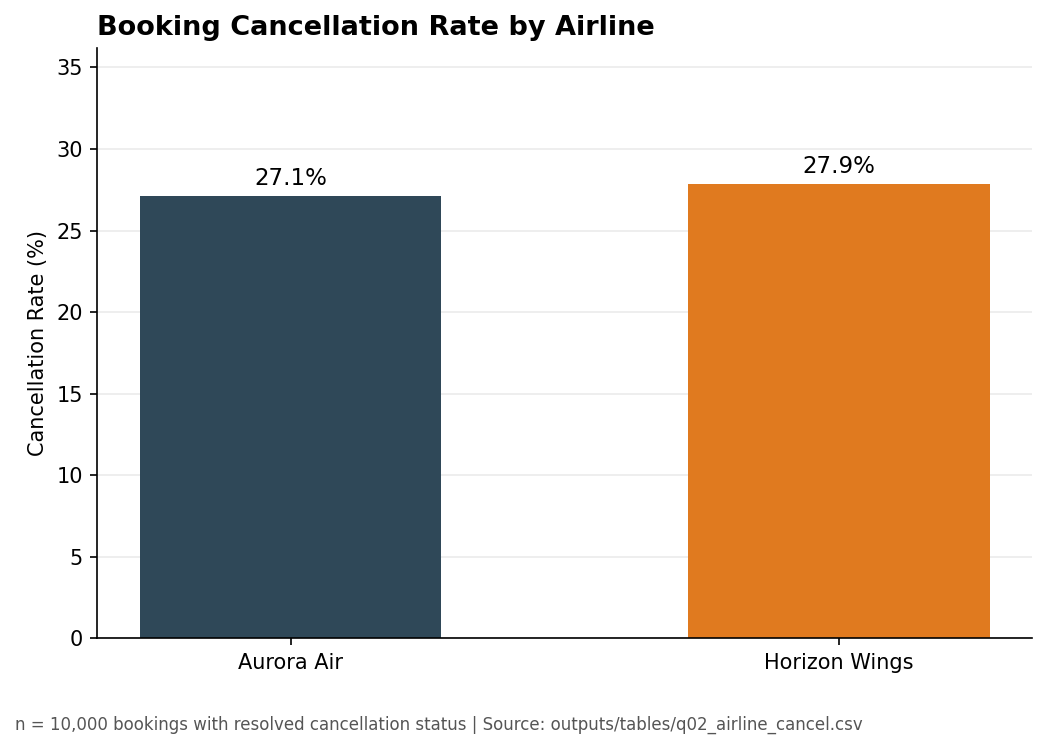
\includegraphics[width=0.85\textwidth]{fig01_airline_cancel}
  \caption{Booking Cancellation Rates for Aurora Air and Horizon Wings}
  \label{fig:q02}
\end{figure}

Empirical results reveal a sharp contrast in booking scale alongside nearly identical cancellation risk across the two airlines:
\begin{itemize}
  \item \textbf{Dominant Market Scale of Aurora Air:} Aurora Air captures \pct{65.22} of total bookings (6,522 bookings), approximately \textbf{1.88 times} the volume of Horizon Wings (3,478 bookings, or \pct{34.78}). This aligns with the broader route network capacity of a Full-Service Carrier.
  \item \textbf{Comparable Cancellation Risk:} Despite differences in service model and customer scale, cancellation rates are nearly identical across both airlines: Horizon Wings records \pct{27.86} while Aurora Air records \pct{27.11} (a difference of only \textbf{0.75 percentage points}).
  \item \textbf{Operational Implication:} An average cancellation rate of roughly 27--28\% poses a sustained challenge to cabin load-factor stability, underscoring the need for calibrated overbooking policies to offset expected seat spoilage.
\end{itemize}

% ---- QUESTION 3 ----
\subsection{Question 3: Monthly Booking Seasonality in 2025}

To isolate true seasonal patterns from partial-year coverage in 2024 and 2026, seasonality analysis is restricted to the 12 full calendar months of 2025 with $N = 5,753$ bookings (Aurora Air: 3,737 bookings; Horizon Wings: 2,016 bookings), verified directly against \code{monthly\_summary.csv}.

\begin{table}[H]
  \centering
  \caption{Bookings by Departure Month in 2025 (\code{q03\_monthly\_departures\_2025.csv})}
  \label{tab:q03}
  \renewcommand{\arraystretch}{1.15}
  \begin{tabular}{llrr}
    \toprule
    \rowcolor{TableHead}
    \textbf{Airline} & \textbf{Month} & \textbf{Bookings} & \textbf{Share of Annual Bookings (\%)} \\
    \midrule
    Aurora Air & January  & 337 & 9.03  \\
    \rowcolor{TableAlt}
    Aurora Air & February  & 299 & 8.01  \\
    Aurora Air & March  & 266 & 7.13  \\
    \rowcolor{TableAlt}
    Aurora Air & April  & 277 & 7.42  \\
    Aurora Air & May  & 300 & 8.04  \\
    \rowcolor{TableAlt}
    Aurora Air & June  & 323 & 8.66  \\
    Aurora Air & \textbf{July}  & \textbf{383} & \textbf{10.27} \\
    \rowcolor{TableAlt}
    Aurora Air & August  & 364 & 9.76  \\
    Aurora Air & September  & 281 & 7.53  \\
    \rowcolor{TableAlt}
    Aurora Air & October & 251 & 6.73  \\
    Aurora Air & November & 268 & 7.18  \\
    \rowcolor{TableAlt}
    Aurora Air & \textbf{December} & \textbf{382} & \textbf{10.24} \\
    \midrule
    Horizon Wings & January  & 165 & 8.19  \\
    \rowcolor{TableAlt}
    Horizon Wings & February  & 160 & 7.94  \\
    Horizon Wings & March  & 146 & 7.25  \\
    \rowcolor{TableAlt}
    Horizon Wings & April  & 154 & 7.64  \\
    Horizon Wings & May  & 142 & 7.05  \\
    \rowcolor{TableAlt}
    Horizon Wings & June  & 172 & 8.54  \\
    Horizon Wings & July  & 189 & 9.38  \\
    \rowcolor{TableAlt}
    Horizon Wings & \textbf{August}  & \textbf{229} & \textbf{11.36} \\
    Horizon Wings & September  & 145 & 7.20  \\
    \rowcolor{TableAlt}
    Horizon Wings & October & 153 & 7.59  \\
    Horizon Wings & November & 150 & 7.44  \\
    \rowcolor{TableAlt}
    Horizon Wings & \textbf{December} & \textbf{210} & \textbf{10.42} \\
    \bottomrule
  \end{tabular}
\end{table}

\begin{figure}[H]
  \centering
  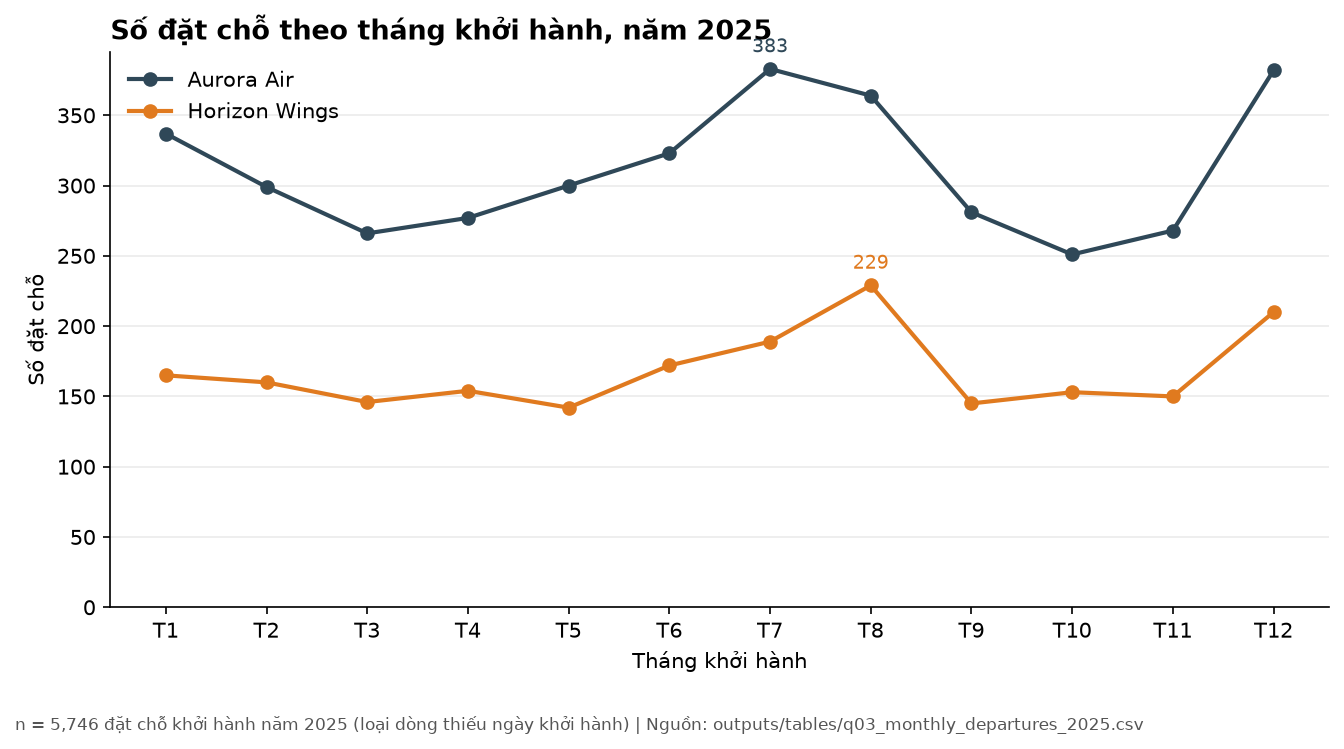
\includegraphics[width=0.90\textwidth]{fig02_monthly_departures_2025}
  \caption{Monthly Booking Trends in 2025}
  \label{fig:q03}
\end{figure}

From Table \ref{tab:q03} and Figure \ref{fig:q03}, two prominent seasonal characteristics emerge:
\begin{itemize}
  \item \textbf{Double-Peak Seasonal Pattern:} Travel demand surges during two distinct windows: the summer holiday peak (July for Aurora Air at 383 bookings; August for Horizon Wings at 229 bookings) and the year-end holiday peak (December with 382 and 210 bookings, respectively).
  \item \textbf{Pronounced Off-Peak Troughs:} Autumn months (September--November) exhibit subdued demand, reaching annual lows in October for Aurora Air (251 bookings, \pct{6.73}) and in May for Horizon Wings (142 bookings, \pct{7.05}).
  \item \textbf{Synchronized Comovement:} Both airlines follow largely parallel monthly trajectories, indicating that demand seasonality is driven primarily by macro-level travel cycles rather than carrier-specific promotions.
\end{itemize}

% ---- QUESTION 4 ----
\subsection{Question 4: Booking Lead Time and Cancellation Risk}

This analysis evaluates $N = 9,978$ bookings with valid \code{booking\_lead\_days} (excluding 22 missing records), with results summarized in Table \ref{tab:q04_stats}, Table \ref{tab:q04_cancel}, and Figure \ref{fig:q04}.

\begin{table}[H]
  \centering
  \caption{Booking Lead Time Statistics by Airline (\code{q04\_leadtime\_stats.csv})}
  \label{tab:q04_stats}
  \renewcommand{\arraystretch}{1.3}
  \begin{tabularx}{\textwidth}{l XXXXXX}
    \toprule
    \rowcolor{TableHead}
    \textbf{Airline} & \textbf{Count (n)} & \textbf{Mean} & \textbf{Median} & \textbf{Q1} & \textbf{Q3} & \textbf{Max.} \\
    \midrule
    Aurora Air    & 6,506 & 71.10 days & 57 days & 27 days & 98 days & 365 days \\
    \rowcolor{TableAlt}
    Horizon Wings & 3,472 & 71.89 days & 58 days & 28 days & 99 days & 365 days \\
    \bottomrule
  \end{tabularx}
\end{table}

\begin{table}[H]
  \centering
  \caption{Cancellation Rates by Booking Lead Time Group (\code{q04\_leadtime\_cancel.csv})}
  \label{tab:q04_cancel}
  \renewcommand{\arraystretch}{1.3}
  \begin{tabularx}{\textwidth}{l XXXX}
    \toprule
    \rowcolor{TableHead}
    \textbf{Lead Time Group (days)} & \textbf{Bookings} & \textbf{Cancelled} & \textbf{Known Status Count} & \textbf{Cancel Rate (\%)} \\
    \midrule
    0--7 days    & 774   & 172   & 774   & 22.22 \\
    \rowcolor{TableAlt}
    8--30 days   & 2,005 & 485   & 2,005 & 24.19 \\
    31--90 days  & 4,327 & 1,115 & 4,327 & 25.77 \\
    \rowcolor{TableAlt}
    91--180 days & 2,276 & 693   & 2,276 & 30.45 \\
    \textbf{181+ days} & \textbf{596} & \textbf{266} & \textbf{596} & \textbf{44.63} \\
    \bottomrule
  \end{tabularx}
\end{table}

\begin{figure}[H]
  \centering
  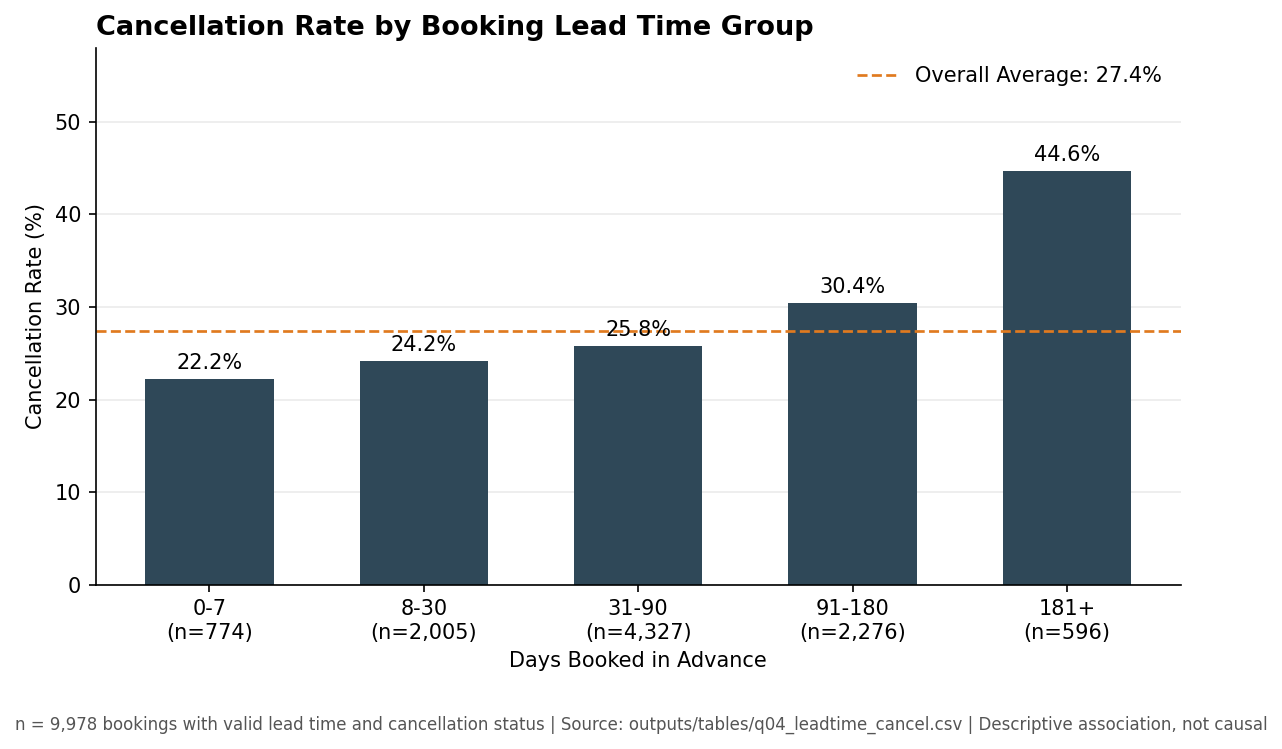
\includegraphics[width=0.85\textwidth]{fig03_leadtime_cancel}
  \caption{Nonlinear Relationship Between Booking Lead Time and Cancellation Rate}
  \label{fig:q04}
\end{figure}

Empirical findings confirm a consistent monotonic pattern: \textbf{longer booking lead times are associated with substantially higher cancellation probabilities}:
\begin{itemize}
  \item Passengers booking close to departure (0--7 days) show the lowest cancellation rate (\pct{22.22}), whereas those booking more than six months in advance (181+ days) exhibit the highest rate at \pct{44.63}.
  \item The cancellation rate in the 181+ day cohort is \textbf{2.01 times} as high (\textbf{+22.41 percentage points}) as that of the 0--7 day cohort, reflecting greater schedule uncertainty over long planning horizons.
\end{itemize}

% ---- QUESTION 5 ----
\subsection{Question 5: International Market Structure --- Top 10 Passenger Countries}

The geographic breakdown spans $N = 9,895$ bookings with valid ISO country codes (excluding 105 missing values) to identify primary source markets across both carriers.

\begin{table}[H]
  \centering
  \caption{Top 10 Passenger Countries by Booking Volume (\code{q05\_top10\_country.csv})}
  \label{tab:q05}
  \renewcommand{\arraystretch}{1.25}
  \begin{tabular}{cc rc}
    \toprule
    \rowcolor{TableHead}
    \textbf{Rank} & \textbf{ISO Alpha-3 Code} & \textbf{Bookings} & \textbf{Booking Share (\%)} \\
    \midrule
    1 & \textbf{VNM (Vietnam)}   & \textbf{2,080} & \textbf{21.02} \\
    \rowcolor{TableAlt}
    2 & CHN (China) & 906   & 9.16  \\
    3 & JPN (Japan)   & 663   & 6.70  \\
    \rowcolor{TableAlt}
    4 & KOR (South Korea)   & 526   & 5.32  \\
    5 & THA (Thailand)   & 515   & 5.20  \\
    \rowcolor{TableAlt}
    6 & USA (United States)     & 489   & 4.94  \\
    7 & SGP (Singapore)  & 398   & 4.02  \\
    \rowcolor{TableAlt}
    8 & AUS (Australia)         & 362   & 3.66  \\
    9 & IND (India)      & 349   & 3.53  \\
    \rowcolor{TableAlt}
    10 & GBR (United Kingdom) & 347 & 3.51 \\
    \bottomrule
  \end{tabular}
\end{table}

\begin{figure}[H]
  \centering
  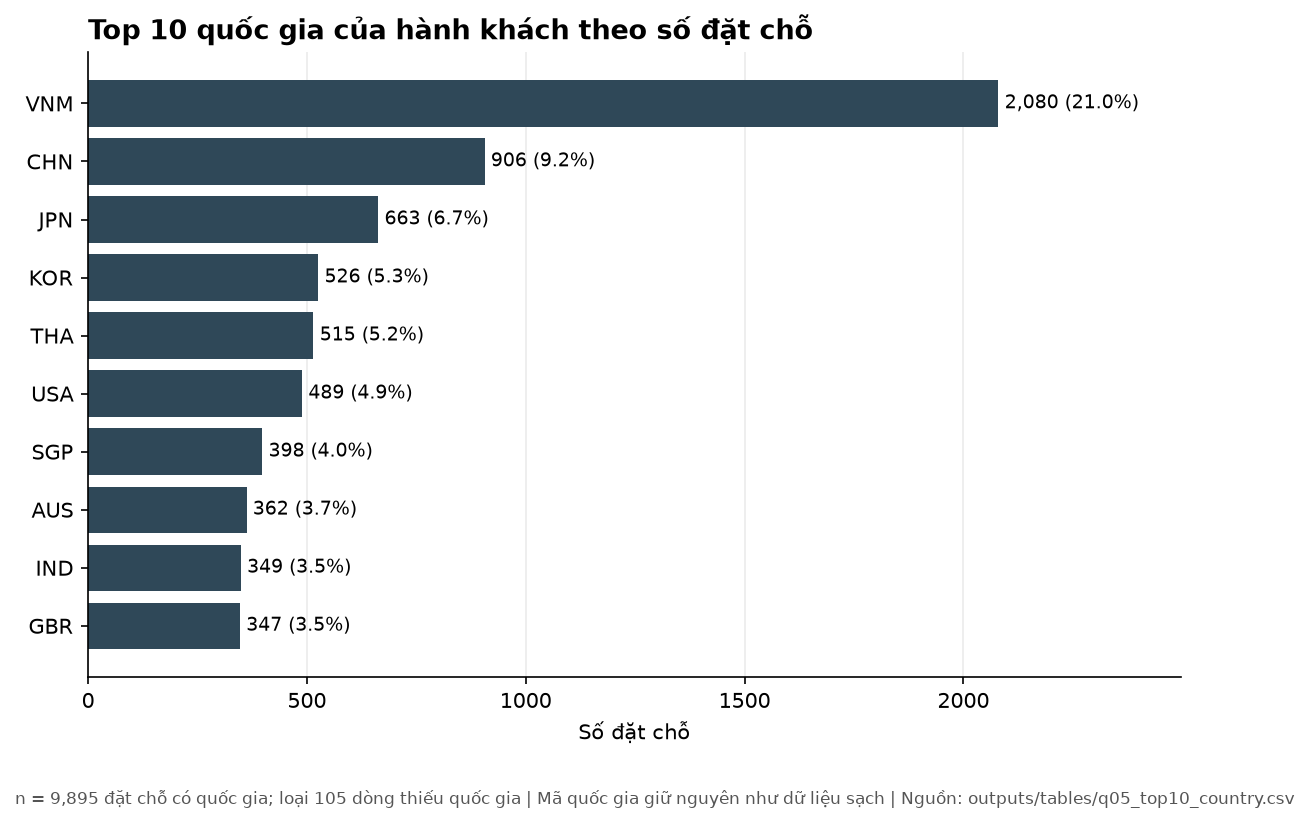
\includegraphics[width=0.85\textwidth]{fig04_top10_country}
  \caption{Booking Volume for the Top 10 Passenger Countries}
  \label{fig:q05}
\end{figure}

Vietnam (VNM) stands as the core domestic market with 2,080 bookings, accounting for \pct{21.02} of total network volume---more than double the second-largest source market, China (906 bookings, 9.16\%). Combined, East and Southeast Asian markets contribute over 47\% of total bookings, supporting a regional network expansion focus.

% ---- QUESTION 6 ----
\subsection{Question 6: Market Segments and Booking Cancellation Risk}

Channel stability across distribution segments is evaluated on $N = 9,968$ bookings with identified market segments (Table \ref{tab:q06} and Figure \ref{fig:q06}).

\begin{table}[H]
  \centering
  \caption{Booking Volume and Cancellation Rate by Market Segment (\code{q06\_segment\_cancel.csv})}
  \label{tab:q06}
  \renewcommand{\arraystretch}{1.3}
  \begin{tabularx}{\textwidth}{l XXXXX}
    \toprule
    \rowcolor{TableHead}
    \textbf{Market Segment} & \textbf{Bookings} & \textbf{Booking Share (\%)} & \textbf{Cancelled} & \textbf{Known Status Count} & \textbf{Cancel Rate (\%)} \\
    \midrule
    Online OTA    & 3,906 & 39.17 & 1,151 & 3,906 & \textbf{29.47} \\
    \rowcolor{TableAlt}
    Group         & 579   & 5.81  & 161   & 579   & 27.81 \\
    Offline Agent & 1,596 & 16.00 & 440   & 1,596 & 27.57 \\
    \rowcolor{TableAlt}
    Direct        & 1,834 & 18.39 & 499   & 1,834 & 27.21 \\
    Loyalty       & 417   & 4.18  & 111   & 417   & 26.62 \\
    \rowcolor{TableAlt}
    Package Tour  & 717   & 7.19  & 174   & 717   & 24.27 \\
    \textbf{Corporate} & \textbf{923} & \textbf{9.26} & \textbf{198} & \textbf{923} & \textbf{21.45} \\
    \bottomrule
  \end{tabularx}
\end{table}

\begin{figure}[H]
  \centering
  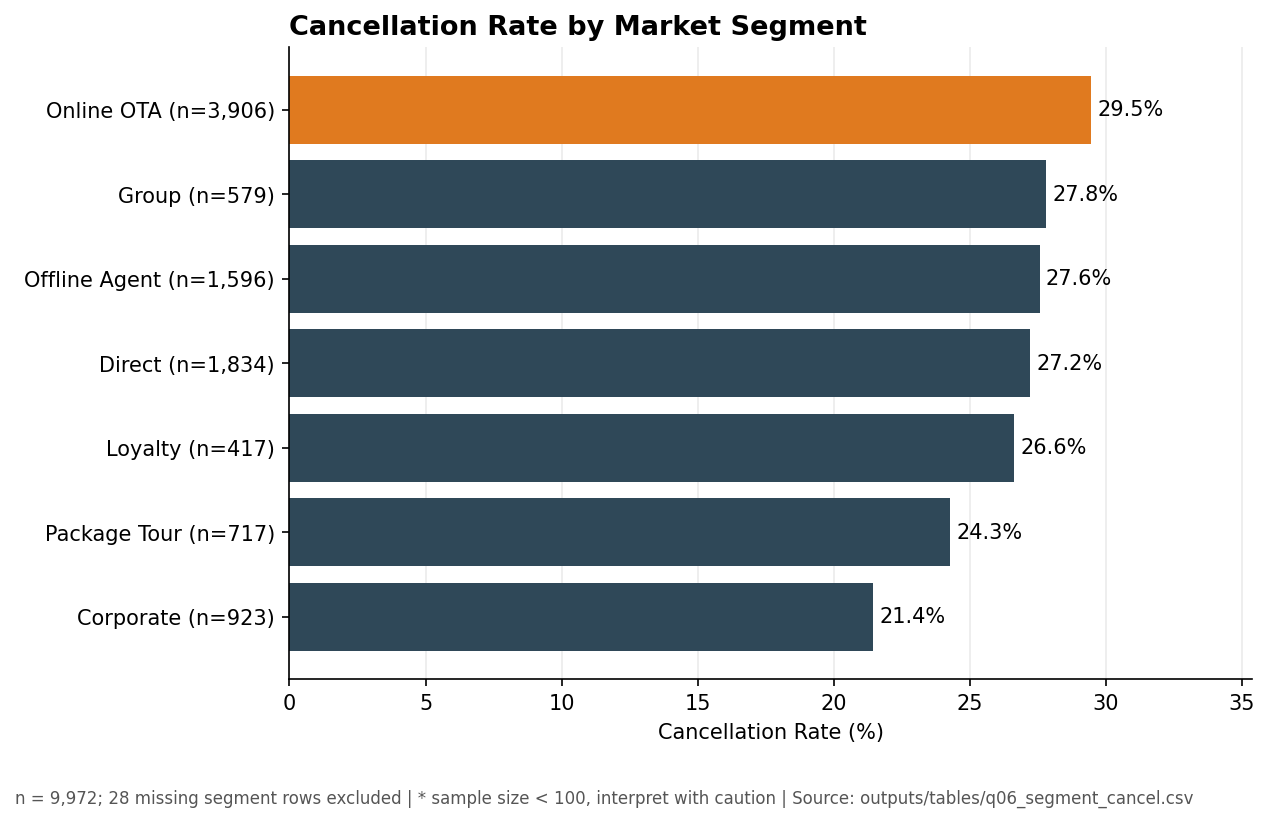
\includegraphics[width=0.88\textwidth]{fig05_segment_cancel}
  \caption{Booking Cancellation Rates by Market Segment}
  \label{fig:q06}
\end{figure}

The \textbf{Online OTA} channel leads decisively in booking volume (\pct{39.17}), yet it simultaneously records the highest cancellation rate in the network (\pct{29.47}). Conversely, the \textbf{Corporate} segment exhibits the strongest booking commitment with a cancellation rate of just \pct{21.45}---\textbf{8.02 percentage points} lower than Online OTA.

% ---- QUESTION 7 ----
\subsection{Question 7: Fare Policy Association with Booking Outcomes}

This section investigates how refund/cancellation rules correlate with final flight status across $N = 9,957$ valid records (Table \ref{tab:q07} and Figure \ref{fig:q07}).

\begin{table}[H]
  \centering
  \caption{Booking Status by Fare Policy (\code{q07\_fare\_policy\_status.csv})}
  \label{tab:q07}
  \renewcommand{\arraystretch}{1.3}
  \begin{tabularx}{\textwidth}{ll XX}
    \toprule
    \rowcolor{TableHead}
    \textbf{Fare Policy} & \textbf{Booking Status} & \textbf{Bookings} & \textbf{Share Within Fare Policy (\%)} \\
    \midrule
    Flexible     & Flown     & 2,519 & 69.91 \\
    \rowcolor{TableAlt}
    Flexible                 & Cancelled   & 1,029 & 28.56 \\
    Flexible                 & No-Show& 55    & 1.53  \\
    \midrule
    Semi-Flexible & Flown         & 2,632 & 71.97 \\
    \rowcolor{TableAlt}
    Semi-Flexible            & Cancelled          & 965   & 26.39 \\
    Semi-Flexible            & No-Show            & 60    & 1.64  \\
    \midrule
    \textbf{Non-Refundable} & \textbf{Flown} & \textbf{2,089} & \textbf{77.26} \\
    \rowcolor{TableAlt}
    Non-Refundable           & Cancelled          & 576   & 21.30 \\
    Non-Refundable           & No-Show            & 39    & 1.44  \\
    \bottomrule
  \end{tabularx}
\end{table}

\begin{figure}[H]
  \centering
  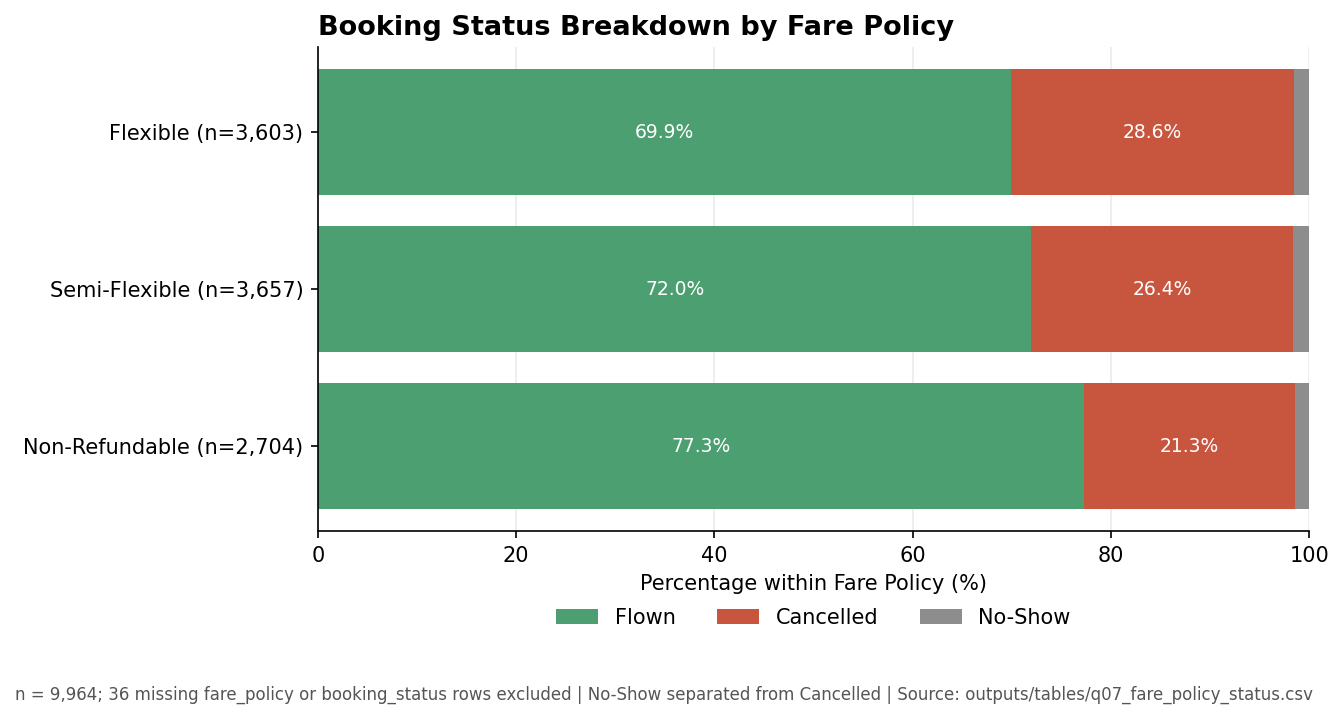
\includegraphics[width=0.88\textwidth]{fig06_fare_policy_status}
  \caption{Booking Status Distribution by Fare Policy}
  \label{fig:q07}
\end{figure}

Financial restrictions align closely with passenger completion behavior: \textbf{Non-Refundable} fares achieve the highest flown rate (\pct{77.26}) and the lowest cancellation rate (\pct{21.30}). By contrast, \textbf{Flexible} fares allow unrestricted refunds and exhibit a substantially higher cancellation rate of \pct{28.56} (\textbf{7.26 percentage points} higher). Notably, \textit{No-Show} rates remain minimal (1.44\%--1.64\%) across all three fare tiers.

% ---- QUESTION 8 ----
\subsection{Question 8: Ticket Fare Analysis by Airline (Non-Cancelled Bookings, Fare $> 0$)}

This comparison examines $N = 7,224$ non-cancelled commercial transactions with strictly positive fares (excluding 9 zero-fare bookings and 30 missing-fare rows) to benchmark pricing across both carriers.

\begin{table}[H]
  \centering
  \caption{Ticket Fare Statistics by Airline (\code{q08\_fare\_stats\_by\_airline.csv})}
  \label{tab:q08}
  \renewcommand{\arraystretch}{1.3}
  \resizebox{\textwidth}{!}{%
  \begin{tabular}{lrrrrrrrcc}
    \toprule
    \rowcolor{TableHead}
    \textbf{Airline} & \textbf{Sample Size (n)} & \textbf{Mean (\$)} & \textbf{Median (\$)} & \textbf{Q1 (\$)} & \textbf{Q3 (\$)} & \textbf{Min (\$)} & \textbf{Max (\$)} & \textbf{Zero-Fare Exclusions} & \textbf{Missing Fares} \\
    \midrule
    Aurora Air    & 4,736 & 208.76 & 149.54 & 123.30 & 190.26 & 56.49 & 2,258.21 & 5 & 13 \\
    \rowcolor{TableAlt}
    Horizon Wings & 2,488 & 194.95 & 135.26 & 112.52 & 171.42 & 48.77 & 2,117.76 & 4 & 17 \\
    \bottomrule
  \end{tabular}}
\end{table}

\begin{figure}[H]
  \centering
  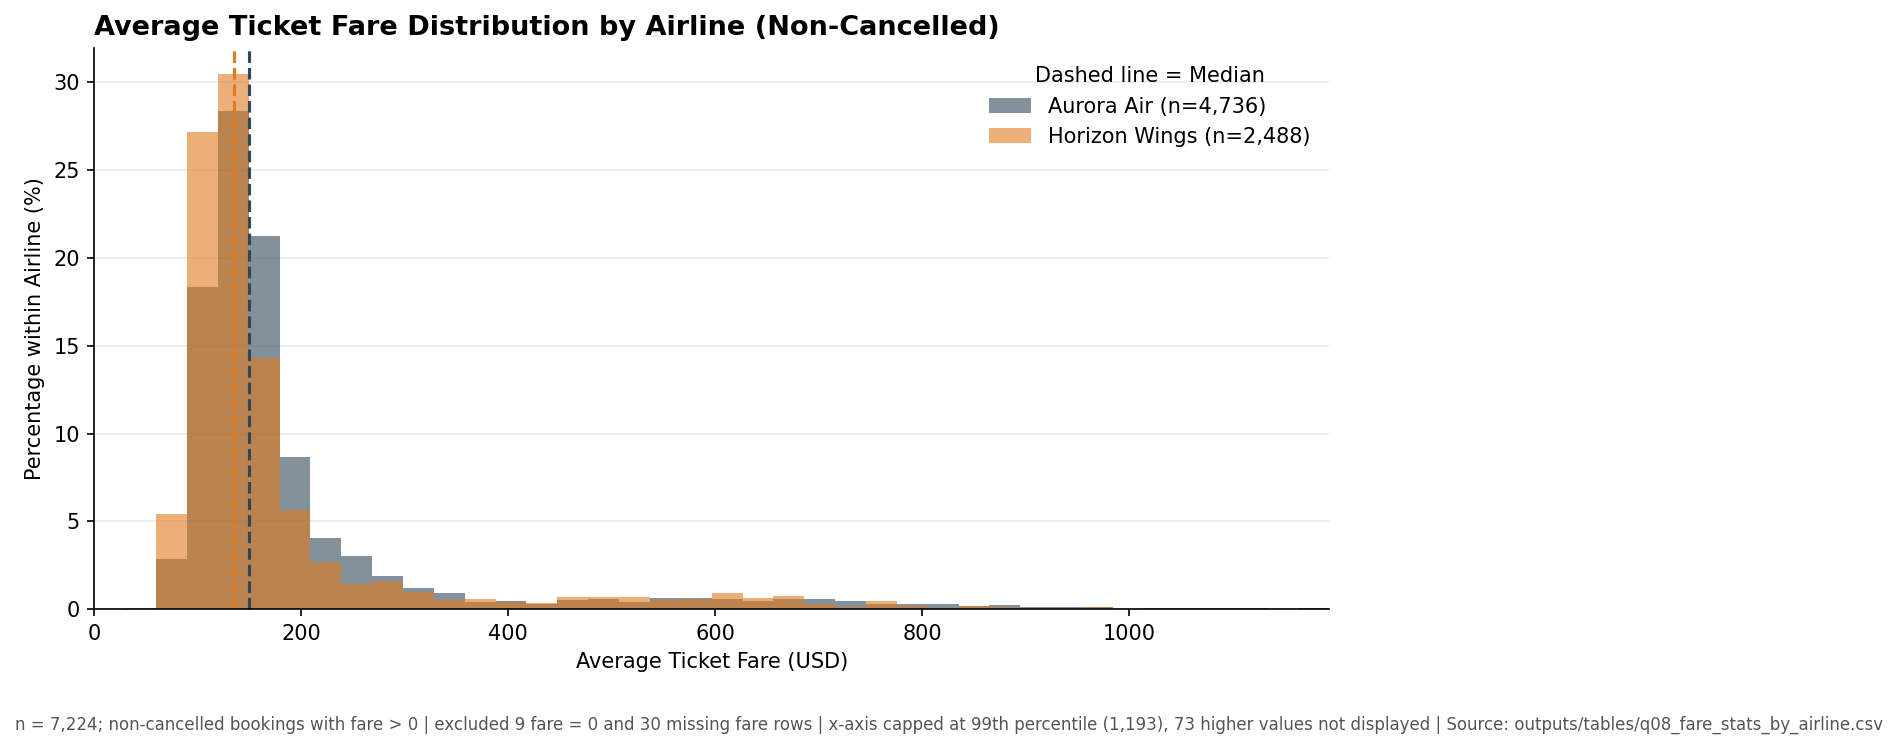
\includegraphics[width=0.88\textwidth]{fig07_fare_hist}
  \caption{Ticket Fare Density by Airline (Truncated at the 99th Percentile)}
  \label{fig:q08}
\end{figure}

Fare distributions exhibit strong positive skewness, with mean fares exceeding medians by 44 to 59 USD for both carriers due to high-value Business and First Class tickets (exceeding 2,200 USD). Consequently, \textbf{the median provides a more representative measure of typical pricing}: Aurora Air's median fare (149.54 USD) exceeds Horizon Wings' median fare (135.26 USD) by \textbf{14.28 USD} (\pct{10.56} higher), consistent with the positioning of a full-service carrier.

% ---- QUESTION 9 ----
\subsection{Question 9: Trip Duration Distribution (Total Trip Days)}

Trip duration (weekend nights plus weeknights) is analyzed across $N = 7,232$ completed itineraries (Aurora Air: 4,733 bookings; Horizon Wings: 2,499 bookings).

\begin{table}[H]
  \centering
  \caption{Passenger Trip Duration Statistics (\code{q09\_trip\_days.csv})}
  \label{tab:q09}
  \renewcommand{\arraystretch}{1.3}
  \begin{tabularx}{\textwidth}{l XXXXXXX}
    \toprule
    \rowcolor{TableHead}
    \textbf{Airline} & \textbf{Count (n)} & \textbf{Mean} & \textbf{Median} & \textbf{Q1} & \textbf{Q3} & \textbf{Max.} & \textbf{Zero-Day Trips} \\
    \midrule
    Aurora Air    & 4,733 & 5.76 days & 4.00 days & 3.00 days & 7.00 days & 45.00 days & 0 \\
    \rowcolor{TableAlt}
    Horizon Wings & 2,499 & 5.95 days & 4.00 days & 3.00 days & 7.00 days & 45.00 days & 0 \\
    \bottomrule
  \end{tabularx}
\end{table}

\begin{table}[H]
  \centering
  \caption{Bookings by Trip Duration Group}
  \label{tab:q09_groups}
  \renewcommand{\arraystretch}{1.3}
  \begin{tabularx}{\textwidth}{X rrrr}
    \toprule
    \rowcolor{TableHead}
    \textbf{Trip Duration Group} & \textbf{Aurora Air (n)} & \textbf{Share (\%)} & \textbf{Horizon Wings (n)} & \textbf{Share (\%)} \\
    \midrule
    1--2 days          & 969   & 20.47 & 500 & 20.01 \\
    \rowcolor{TableAlt}
    \textbf{3--4 days} & \textbf{1,540} & \textbf{32.54} & \textbf{776} & \textbf{31.05} \\
    5--7 days          & 1,253 & 26.47 & 678 & 27.13 \\
    \rowcolor{TableAlt}
    8--14 days         & 725   & 15.32 & 407 & 16.29 \\
    15+ days           & 246   & 5.20  & 138 & 5.52  \\
    \bottomrule
  \end{tabularx}
\end{table}

\begin{figure}[H]
  \centering
  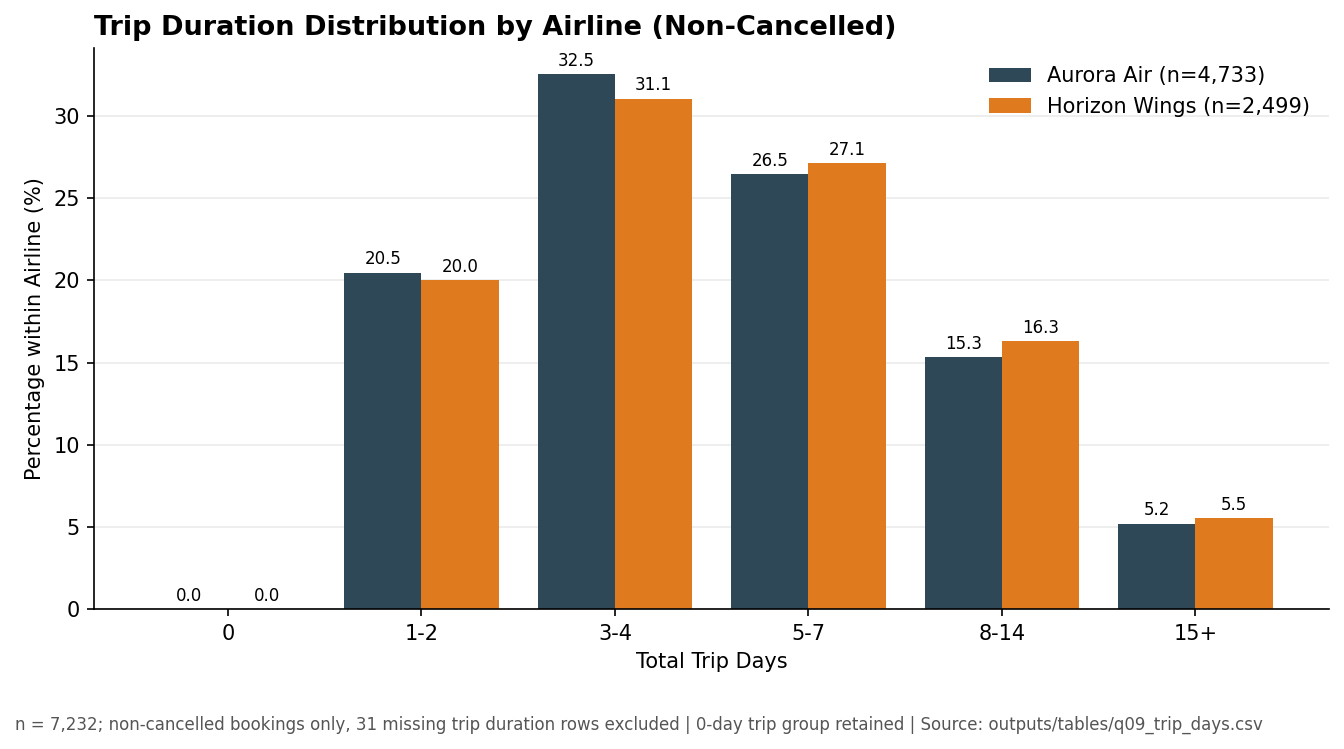
\includegraphics[width=0.88\textwidth]{fig08_trip_days}
  \caption{Passenger Trip Duration Distribution}
  \label{fig:q09}
\end{figure}

Nearly 80\% of passengers undertake trips lasting 1 to 7 days, with the \textbf{3--4 day} duration bracket accounting for the largest single share ($\sim$31--32\%). This pattern reflects strong demand from short-break leisure travelers and weekly business itineraries.

% ---- QUESTION 10 ----
\subsection{Question 10: Cabin Class Change Rates}

Seating assignment consistency is measured across $N = 9,921$ bookings containing valid codes for both booked cabin and assigned cabin (Table \ref{tab:q10_airline} and Table \ref{tab:q10_cabin}).

\begin{table}[H]
  \centering
  \caption{Cabin Change Rates by Airline (\code{q10\_cabin\_change\_by\_airline.csv})}
  \label{tab:q10_airline}
  \renewcommand{\arraystretch}{1.3}
  \begin{tabularx}{\textwidth}{l XXX}
    \toprule
    \rowcolor{TableHead}
    \textbf{Airline} & \textbf{Valid Sample Size (n)} & \textbf{Cabin Changes} & \textbf{Cabin Change Rate (\%)} \\
    \midrule
    Aurora Air    & 6,472 & 737 & 11.39 \\
    \rowcolor{TableAlt}
    Horizon Wings & 3,449 & 405 & 11.74 \\
    \bottomrule
  \end{tabularx}
\end{table}

\begin{table}[H]
  \centering
  \caption{Cabin Change Rates by Booked Cabin Code (\code{q10\_cabin\_change\_by\_booked\_code.csv})}
  \label{tab:q10_cabin}
  \renewcommand{\arraystretch}{1.25}
  \begin{tabularx}{\textwidth}{l rrr >{\raggedright\arraybackslash}X}
    \toprule
    \rowcolor{TableHead}
    \textbf{Booked Cabin Code} & \textbf{Count (n)} & \textbf{Cabin Changes} & \textbf{Change Rate (\%)} & \textbf{Sample Notes} \\
    \midrule
    B1 & 314   & 37  & 11.78 & Standard Sample ($n > 100$) \\
    \rowcolor{TableAlt}
    B2 & 247   & 32  & 12.96 & Standard Sample ($n > 100$) \\
    \textbf{B3} & \textbf{177} & \textbf{24} & \textbf{13.56} & \textbf{Highest Rate} \\
    \rowcolor{TableAlt}
    E1 & 2,323 & 257 & 11.06 & Large Sample \\
    E2 & 2,363 & 283 & 11.98 & Large Sample \\
    \rowcolor{TableAlt}
    E3 & 1,923 & 204 & 10.61 & Large Sample \\
    E4 & 1,470 & 185 & 12.59 & Large Sample \\
    \rowcolor{TableAlt}
    F1 & 55    & 7   & 12.73 & \textcolor{AccentRed}{Caution: $n < 100$} \\
    F2 & 34    & 3   & 8.82  & \textcolor{AccentRed}{Caution: $n < 100$} \\
    \rowcolor{TableAlt}
    F3 & 38    & 4   & 10.53 & \textcolor{AccentRed}{Caution: $n < 100$} \\
    P1 & 530   & 61  & 11.51 & Standard Sample ($n > 100$) \\
    \rowcolor{TableAlt}
    P2 & 447   & 45  & 10.07 & Standard Sample ($n > 100$) \\
    \bottomrule
  \end{tabularx}
\end{table}

Seating operations remain broadly stable, with roughly \pct{89} of passengers accommodated in their originally booked cabin class. Cabin reassignments are most prevalent among Business Class bookings (\textbf{B3} at \pct{13.56} and \textbf{B2} at \pct{12.96}), reflecting operational seat reallocations and upgrades designed to balance cabin capacity across flights.

% =========================================================
\section{Synthesis of Six Key Business Insights}
% =========================================================

Table \ref{tab:insights_summary} synthesizes six strategic empirical findings supporting airline revenue management decisions.

\begin{table}[H]
  \centering
  \caption{Six Key Business Findings}
  \label{tab:insights_summary}
  \renewcommand{\arraystretch}{1.4}
  \begin{tabularx}{\textwidth}{c XXX}
    \toprule
    \rowcolor{TableHead}
    \textbf{\#} & \textbf{Analysis Topic} & \textbf{Supporting Evidence} & \textbf{Key Finding} \\
    \midrule
    \textbf{1} & Booking Lead Time
      & Table \ref{tab:q04_cancel}, Figure \ref{fig:q04}
      & Cancellation rates rise nonlinearly with lead time, peaking at 44.63\% for bookings made more than six months in advance. \\
    \rowcolor{TableAlt}
    \textbf{2} & Fare Policy
      & Table \ref{tab:q07}, Figure \ref{fig:q07}
      & Non-refundable fares have the highest flown rate (77.26\%) and the lowest cancellation rate (21.30\%). \\
    \textbf{3} & Market Segment
      & Table \ref{tab:q06}, Figure \ref{fig:q06}
      & Online OTAs account for the largest booking share (39.17\%) and have the highest cancellation rate (29.47\%). \\
    \rowcolor{TableAlt}
    \textbf{4} & Seasonality
      & Table \ref{tab:q03}, Figure \ref{fig:q03}
      & Demand for both airlines peaks in summer and December. \\
    \textbf{5} & Fare Positioning
      & Table \ref{tab:q08}, Figure \ref{fig:q08}
      & Fares are strongly right-skewed. Aurora Air's median fare is 10.56\% higher than Horizon Wings'. \\
    \rowcolor{TableAlt}
    \textbf{6} & Cabin Changes
      & Table \ref{tab:q10_cabin}
      & The cabin change rate averages $\sim$11.5\% and is highest in business class (13.56\% for B3). \\
    \bottomrule
  \end{tabularx}
\end{table}

Detailed interpretations of each key finding are presented below:

\begin{insightbox}{Insight 1: Booking Lead Time and Nonlinear Escalation of Cancellation Risk}
Analyzing 9,978 transactions with valid lead-time data highlights a clear inverse relationship between booking horizon and itinerary certainty. Passengers booking close to departure (0--7 days) record a cancellation rate of only \pct{22.22}, whereas cancellations climb progressively through 8--30 days (\pct{24.19}) and 31--90 days (\pct{25.77}) before accelerating sharply to \pct{44.63} for bookings made over six months ahead (181+ days). Bookings made more than six months in advance are cancelled at \textbf{2.01 times} the rate (+22.41 percentage points) of last-week bookings.

\textit{Business Implication:} Early shoppers frequently lock in promotional inventory before travel plans are firm, inflating speculative reservations across inventory systems. Airlines should introduce staged deposit requirements or stricter ticketing time limits for reservations created more than 90 days prior to departure.
\end{insightbox}

\begin{insightbox}{Insight 2: Financial Commitments in Fare Policies Align with Passenger Retention}
Across 9,957 bookings, ticket refundability rules correspond strongly to final flight completion outcomes. \textbf{Non-Refundable} fares achieve the highest flown rate across the network at \pct{77.26} (2,089 of 2,704 bookings) alongside the lowest cancellation rate (\pct{21.30}). Conversely, \textbf{Flexible} fares reach a \pct{28.56} cancellation rate---\textbf{7.26 percentage points} higher than Non-Refundable tickets. Across all three fare policies, \textit{No-Show} rates remain consistently low (1.4\%--1.6\%).

\textit{Business Implication:} Monetary forfeiture risk reinforces traveler commitment to confirmed itineraries. Carriers can rebalance seat capacity protection against customer flexibility by expanding well-calibrated Semi-Flexible fare tiers rather than offering overly permissive Flexible allotments.
\end{insightbox}

\begin{insightbox}{Insight 3: The Online OTA Paradox --- Highest Volume Accompanied by Highest Cancellation Risk}
Among 9,968 bookings with known segments, the \textbf{Online OTA} channel generates the largest share of reservations at \pct{39.17} (3,906 bookings). At the same time, it carries the highest cancellation risk across the network at \pct{29.47} (1,151 cancellations). This rate stands well above both the \textbf{Corporate} segment---which posts the lowest cancellation rate at \pct{21.45} (a gap of \textbf{8.02 percentage points})---and the \textbf{Direct} channel (\pct{27.21}).

\textit{Business Implication:} Metasearch and price-comparison workflows on OTA platforms make it frictionless for travelers to hold duplicate seats or switch to cheaper departures close to travel dates. Airlines should tighten Service Level Agreements (SLAs) with OTA partners and shorten unpaid hold windows to curb speculative bookings.
\end{insightbox}

\begin{insightbox}{Insight 4: Synchronized Double-Peak Seasonality Requires Agile Capacity Management}
Evaluation of 5,753 departures in calendar year 2025 confirms a synchronized two-peak demand cycle across both airlines: a summer travel peak (July--August) and a year-end holiday peak (December). Peak-month booking volume reaches \textbf{1.53 times} the lowest-month volume for Aurora Air (383 vs.\ 251 bookings) and \textbf{1.61 times} for Horizon Wings (229 vs.\ 142 bookings).

\textit{Business Implication:} Parallel seasonal swings indicate shared market-wide travel cycles. Revenue teams should deploy active \textit{Dynamic Pricing} during summer and December peaks while scheduling planned fleet maintenance and crew training during off-peak troughs in May and October.
\end{insightbox}

\begin{insightbox}{Insight 5: Right-Skewed Fare Distribution and Carrier Market Positioning}
Across 7,224 non-cancelled positive-fare transactions, ticket pricing exhibits strong right skewness driven by Business and First Class fares exceeding 2,100 USD. Accordingly, the median serves as the primary benchmark for typical ticket pricing: Aurora Air's median fare of \textbf{149.54 USD} surpasses Horizon Wings' median of \textbf{135.26 USD} by \textbf{14.28 USD} (a \pct{10.56} premium).

\textit{Business Implication:} The median price differential reflects distinct competitive positioning between a full-service carrier and a cost-optimized challenger. Because ancillary fees (baggage, seat selection, meals) are not captured in the base fare field, Horizon Wings may narrow effective yield differences through targeted ancillary bundling.
\end{insightbox}

\begin{insightbox}{Insight 6: High Overall Cabin Stability with Elevated Reassignment in Business Class}
Analysis of 9,921 bookings shows comparable cabin-change rates for Aurora Air (\pct{11.39}) and Horizon Wings (\pct{11.74}), averaging roughly 11.5\%---indicating that nearly 89\% of travelers receive seats in their originally booked cabin. Cabin reassignments occur most frequently in Business Class bookings, led by \textbf{B3} (\pct{13.56}) and \textbf{B2} (\pct{12.96}), nearly 3 percentage points higher than Economy sub-class E3 (\pct{10.61}).

\textit{Business Implication:} Elevated reassignment rates in Business fare buckets likely reflect operational upgrades, cabin swaps, or inventory rebalancing during peak Economy demand. Standardizing upgrade allocation rules around loyalty status can boost customer satisfaction without inflating operating costs.
\end{insightbox}

% =========================================================
\chapter{DATA LIMITATIONS \& MANAGERIAL RECOMMENDATIONS}
% =========================================================

\section{Study Limitations}

The research team notes several methodological and structural limitations inherent to the dataset:
\begin{enumerate}
  \item \textbf{Simulated Dataset Design:} The dataset was synthetically constructed for data-cleaning evaluation and quantitative analytics practice. Observed statistical associations reflect the underlying data-generation process and cannot establish causal mechanisms or be directly generalized to live airline operations without real-world validation.
  \item \textbf{Incomplete Multi-Year Coverage:} Across the 26-month observation window (July 2024 to August 2026), only calendar year 2025 spans all 12 complete months. Seasonality analysis was therefore scoped strictly to 2025 to prevent edge-month sampling distortion, precluding formal Year-over-Year (YoY) growth comparisons.
  \item \textbf{Absence of Operating Cost and Ancillary Revenue Fields:} The \code{avg\_ticket\_fare} field measures nominal base ticket value only and omits ancillary revenues (baggage, meals, seat fees) as well as variable operating expenses (fuel, crew, airport charges). Consequently, \code{booking\_value\_est} represents nominal gross booking value rather than flight net profit.
\end{enumerate}

\section{Managerial Recommendations for Airlines}

Grounded in the empirical findings above, the team proposes four strategic actions for airline Revenue Management:

\begin{itemize}
  \item \textbf{Control Cancellation Risk on Long-Lead Bookings (Lead Time $>$ 90 Days):} Implement progressive payment schedules or tiered cancellation fees scaled by booking horizon for reservations created more than three months before departure to deter speculative seat holding.
  \item \textbf{Optimize Online OTA Channel Governance:} Shorten unpaid reservation hold windows for Online OTA bookings to within 24 hours of PNR creation, while introducing targeted digital perks or loyalty discounts to shift repeat travelers toward direct airline websites and mobile apps.
  \item \textbf{Deploy Seasonality-Adaptive Pricing and Packaging:} Calibrate \textit{Dynamic Pricing} rules to capture peak willingness-to-pay during the July--August and December surges, while partnering with tour operators on bundled \textit{Package Tour} promotions to stimulate load factors during May and October troughs.
  \item \textbf{Monetize Short-Trip Segments Through Convenience Bundles:} Because over 50\% of passengers travel for 1 to 4 days, airlines should promote fast-track add-on bundles (priority boarding, extra cabin baggage, express airport transfers) tailored to time-sensitive leisure and corporate short-haul travelers.
\end{itemize}

% =========================================================

\end{document}

